% ==============================================================================
% METODOLOGÍA
% ==============================================================================
% Instrucciones de la plantilla:
% - Presentar de manera clara y estructurada el proceso seguido durante la práctica de laboratorio.
% - Comenzar con la configuración del entorno de trabajo.
% - Detallar los algoritmos gráficos implementados explicando su fundamento teórico y su adaptación práctica.
% - Incluir imágenes con títulos y descripciones de los pasos ejecutados.
% - Suficientemente detallado para que cualquier lector pueda replicar el programa.
% - REGLA: "Una metodología por actividad".
% ==============================================================================

\section{Metodología}

\subsection{Configuración del entorno de trabajo}
En la Tabla \ref{tab:requerimientos} se resumen las herramientas empleadas. El proyecto de OpenGL es el \texttt{06\_Texturing} del repositorio del laboratorio, que ya incluye la clase \texttt{Model} (\texttt{model.h}) basada en Assimp, un \textit{shader} que dibuja únicamente el color de la textura y un cubo de entorno (\texttt{mycube.fbx}).

\begin{table}[H]
\centering
\renewcommand{\arraystretch}{1.25}
\begin{tabular}{|p{4.2cm}|p{10.5cm}|}
\hline
\textbf{Elemento} & \textbf{Especificación / Versión empleada} \\ \hline
Sistema operativo & Windows 11 (64 bits) \\ \hline
Entorno de desarrollo & Microsoft Visual Studio Community (conjunto de herramientas \texttt{v145}) \\ \hline
Compilador y estándar & MSVC, \texttt{C++20}, configuración \texttt{Debug|x64} \\ \hline
API gráfica & OpenGL 3.3 (perfil núcleo) \\ \hline
Bibliotecas & GLFW, GLAD, GLM, Assimp (\texttt{assimp-vc143-mtd}) y \texttt{stb\_image} \\ \hline
Modelado y texturas & Blender 5.2.2 LTS con guiones en Python (\texttt{bpy}, \texttt{bmesh}, NumPy) \\ \hline
\end{tabular}
\caption{Herramientas, bibliotecas y versiones utilizadas.}
\label{tab:requerimientos}
\end{table}

\subsubsection{Creación del proyecto en Visual Studio}
Como en las prácticas anteriores, dentro de la carpeta \texttt{06\_Texturing} se creó la carpeta del proyecto \texttt{Proyecto06} con la plantilla \textit{Proyecto vacío} de C++, se agregaron los archivos \texttt{06\_Texturing.cpp} y \texttt{stb\_image.cpp}, y se configuraron las propiedades de la Tabla \ref{tab:propiedades} para las configuraciones \texttt{Debug|x64} y \texttt{Release|x64}. Además de GLFW y GLAD, que indica el manual, fue necesario agregar Assimp, porque \texttt{model.h} incluye \texttt{<assimp/Importer.hpp>}: sin esa biblioteca el proyecto compila pero no enlaza.

\begin{table}[H]
\centering
\renewcommand{\arraystretch}{1.25}
\begin{tabular}{|p{5.2cm}|p{9.5cm}|}
\hline
\textbf{Propiedad} & \textbf{Valor} \\ \hline
Directorio de salida y de trabajo & \texttt{\$(ProjectDir)..\textbackslash..\textbackslash bin\textbackslash} \\ \hline
Directorios de inclusión adicionales & \texttt{deps\textbackslash glm}, \texttt{deps\textbackslash glad}, \texttt{deps\textbackslash glfw}, \texttt{deps\textbackslash assimp} e \texttt{include} del proyecto \\ \hline
Directorios de bibliotecas adicionales & \texttt{deps\textbackslash glad}, \texttt{deps\textbackslash glfw} y \texttt{deps\textbackslash assimp} (\texttt{lib\textbackslash x64\textbackslash Debug}) \\ \hline
Dependencias adicionales & \texttt{opengl32.lib; glad.lib; glfw3.lib; assimp-vc143-mtd.lib} \\ \hline
Definiciones del preprocesador & \texttt{\_CRT\_SECURE\_NO\_WARNINGS} (por \texttt{stb\_image}) \\ \hline
\end{tabular}
\caption{Propiedades del proyecto \texttt{Proyecto06} en Visual Studio.}
\label{tab:propiedades}
\end{table}

\subsubsection{Procedimiento común en Blender}
Todo el trabajo en Blender quedó escrito en guiones de Python, uno por actividad y guardados en la carpeta \texttt{codigo} (\texttt{plano\_act1.py}, \texttt{caja\_act2.py}, \texttt{barril\_act3.py}, \texttt{planeta\_act4.py} y \texttt{variaciones.py}), que se ejecutan sobre el mismo archivo \texttt{.blend} con Blender abierto, de manera que cada objeto nuevo se agrega a la escena sin borrar los anteriores. Las texturas se construyen como arreglos de NumPy a partir de las fotografías, se escriben en una imagen de Blender y se guardan en PNG. Todas miden potencias de dos, y la Tabla \ref{tab:texturas} resume de qué imágenes se forma cada una.

\begin{table}[H]
\centering
\renewcommand{\arraystretch}{1.2}
\begin{tabular}{|p{2.6cm}|p{2.3cm}|p{9.6cm}|}
\hline
\textbf{Textura} & \textbf{Tamaño} & \textbf{Imágenes que combina} \\ \hline
Hoja & $1024^2$ RGBA & Foto de una hoja \cite{hoja_commons} + canal alfa calculado \\ \hline
Caja & $2048^2$ & Cartón kraft \cite{carton_commons} + pestaña y cinta \\ \hline
Barril & $2048^2$ & Duelas \texttt{Planks005} + aros \texttt{Metal021} + tapas \texttt{Planks012} \cite{ambientcg} \\ \hline
Planeta & $2048 \times 1024$ & Mapa diurno de la Tierra \cite{solarsystemscope} \\ \hline
Reja & $1024^2$ RGBA & \texttt{Metal011} \cite{ambientcg} + malla de rombos calculada como canal alfa \\ \hline
Edificio & $2048^2$ & \texttt{Bricks005} + \texttt{Concrete006} + \texttt{Planks012} \cite{ambientcg} + cielo del cubemap \cite{humus} \\ \hline
Tinaco & $1024^2$ & \texttt{Plastic006} \cite{ambientcg} + estrías y rosca \\ \hline
Balón & $2048 \times 1024$ & \texttt{Leather012} \cite{ambientcg} + patrón del icosaedro truncado \\ \hline
\end{tabular}
\caption{Texturas de la práctica, su tamaño y las imágenes que se combinaron en cada una.}
\label{tab:texturas}
\end{table}

% ------------------------------------------------------------------------------
\subsection{Actividad 1: Textura en un plano}

\subsubsection{Selección de la imagen}
Para que el plano mostrara algo más que una imagen rectangular decidimos usar una textura con transparencia: una hoja recortada sobre un fondo transparente, que en OpenGL deja ver el escenario alrededor de su contorno. La fotografía que elegimos \cite{hoja_commons} (Figura \ref{fig:hoja_original}) mide $719 \times 717$ píxeles y, al revisar el encabezado del PNG, encontramos que su tipo de color es 2 (RGB), es decir, no trae canal alfa: había que generarlo nosotros.

\begin{figure}[H]
    \centering
    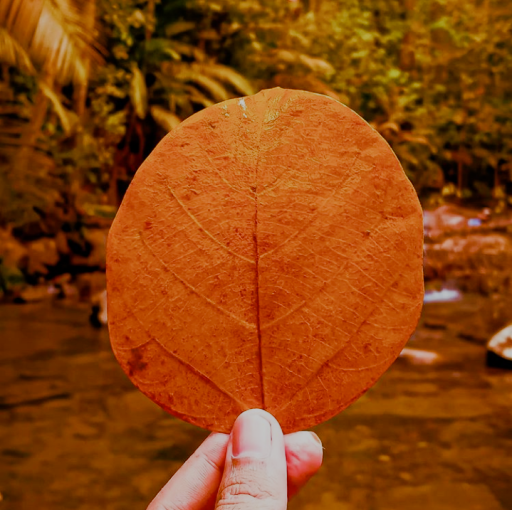
\includegraphics[width=0.38\textwidth]{Imagenes/E1/01_hoja_original.png}
    \caption{Fotografía original de la hoja ($719 \times 717$, RGB, sin canal alfa).}
    \label{fig:hoja_original}
\end{figure}

\subsubsection{Generación del canal alfa}
El guion \texttt{plano\_act1.py} recorta la foto a $717 \times 717$ para hacerla cuadrada y calcula el alfa con los pasos siguientes:
\begin{enumerate}
    \item \textbf{Umbral de color.} La hoja es un naranja muy saturado, así que se marcan los píxeles con $R > 0.55$, $G < 0.62R$ y $B < 0.30R$.
    \item \textbf{Apertura morfológica.} Tres erosiones seguidas de tres dilataciones cortan los puentes delgados que unen la hoja con manchas del fondo del mismo color.
    \item \textbf{Región conexa.} Se conserva solo la región conectada a un píxel del centro de la hoja, $(371, 360)$, mediante dilataciones repetidas.
    \item \textbf{Límite elíptico.} Se descarta todo lo que queda fuera de una elipse un 4\,\% más grande que la hoja (centro $(371, 364)$ y semiejes $223 \times 242$).
    \item \textbf{Relleno por filas.} Cada fila se llena entre su primer y su último píxel marcado, lo que recupera la vena central, los brillos y la punta, que no pasan el umbral.
    \item \textbf{Piel.} Se quitan los píxeles con $B > 0.6R$, que corresponden al pulgar que sostiene la hoja.
    \item \textbf{Orilla suave.} Dos pasadas de un promedio de $3 \times 3$ convierten la orilla en una transición de unos dos píxeles.
\end{enumerate}
Finalmente la imagen se escala a $1024 \times 1024$ y se guarda como PNG RGBA. La Figura \ref{fig:hoja_rgba} muestra el resultado compuesto sobre un fondo magenta para hacer visible la transparencia: el 33\,\% de los píxeles quedó opaco.

\begin{lstlisting}[language=Python, caption={Núcleo del cálculo del canal alfa en plano\_act1.py.}, label={lst:mascara_hoja}]
m = (R > 0.55) & (G < 0.62 * R) & (B < 0.30 * R)      # naranja saturado
for _ in range(APERTURA):                               # apertura: separa del fondo
    m = _vecinos(m, np.logical_and)
m = _inundar(semilla, m)                                # region conectada al centro
for _ in range(APERTURA):
    m = _vecinos(m, np.logical_or)
m &= d < LIMITE                                         # elipse 4 % mayor que la hoja
for f in range(LADO):                                   # relleno de orilla a orilla
    xs = np.flatnonzero(m[f])
    if xs.size:
        m[f, xs[0]:xs[-1] + 1] = True
m &= ~((B > 0.6 * R) & (R > 0.6))                       # piel del pulgar
\end{lstlisting}

\begin{figure}[H]
    \centering
    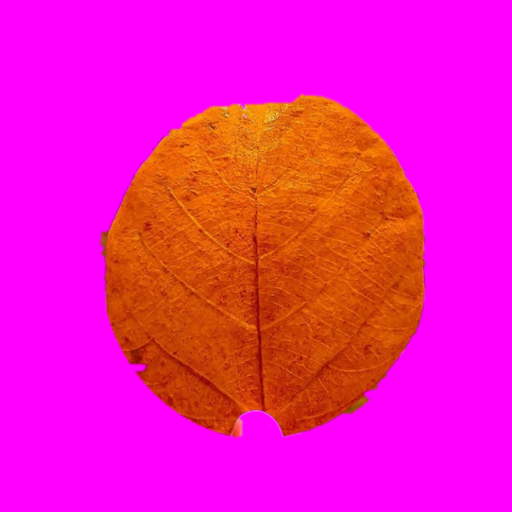
\includegraphics[width=0.38\textwidth]{Imagenes/E1/02_hoja_rgba_magenta.png}
    \caption{Textura \texttt{hoja\_rgba.png} ($1024 \times 1024$, RGBA) compuesta sobre magenta: lo magenta es la parte transparente.}
    \label{fig:hoja_rgba}
\end{figure}

\subsubsection{Plano y material}
El plano es un \textit{Plane} de 2 unidades por lado en el origen, cuyas coordenadas UV ya cubren el cuadrado $[0, 1]^2$. Su material conecta un nodo \textit{Image Texture} con la hoja a las entradas \textit{Base Color} y \textit{Alpha} del \textit{Principled BSDF}, y usa el método de \textit{render} \textit{Blended} para que la vista de Blender muestre la transparencia. El plano se exportó a \texttt{Blender/plano\_hoja.fbx}.

% ------------------------------------------------------------------------------
\subsection{Actividad 2: Cubo como caja de cartón}

\subsubsection{Atlas de la caja}
Partimos de una fotografía de cartón kraft liso \cite{carton_commons}, recortada a cuadrado y reducida a $512 \times 512$. Con ella se arma un atlas de $2048 \times 2048$ dividido en una cuadrícula de $4 \times 4$ celdas de 512 píxeles, de las que se usan seis, una por cara (Figura \ref{fig:atlas_caja}). A cada celda se le oscurecen las orillas un 25\,\% para marcar las aristas de la caja; la tapa y el fondo llevan la línea donde se juntan las pestañas y encima una cinta canela que ocupa el 20\,\% de la celda, y en las dos caras laterales $\pm X$ la cinta baja un 28\,\% de la altura, justo donde termina la de la tapa.

\subsubsection{Coordenadas UV por cara}
El cubo es de 2 unidades por lado y está apoyado en el piso en $(3, 0, 1)$. El guion \texttt{caja\_act2.py} recorre las caras con \texttt{bmesh} y, según la normal de cada una, proyecta sus vértices sobre los dos ejes de la cara con la orientación que deja el «arriba» de los costados hacia $+Z$; después lleva el resultado a su celda dejando un margen de 4 píxeles para que el filtrado no tome color de la celda vecina:
\begin{equation}
    u = \frac{c + m + \frac{a+1}{2}(1 - 2m)}{4}, \qquad v = \frac{f + m + \frac{b+1}{2}(1 - 2m)}{4},
\end{equation}
donde $(a, b) \in [-1, 1]^2$ es la proyección del vértice sobre la cara, $(c, f)$ la columna y fila de la celda y $m = 4/512$ el margen.

\begin{lstlisting}[language=Python, caption={Asignación de las coordenadas UV de cada cara en caja\_act2.py.}, label={lst:uv_caja}]
CARAS = {
    (0, -1, 0): ((0, 0), lambda x, y, z: (x, z)),     # frente
    (1, 0, 0):  ((1, 0), lambda x, y, z: (y, z)),     # derecha
    (0, 1, 0):  ((2, 0), lambda x, y, z: (-x, z)),    # atras
    (-1, 0, 0): ((0, 1), lambda x, y, z: (-y, z)),    # izquierda
    (0, 0, 1):  ((1, 1), lambda x, y, z: (x, y)),     # tapa
    (0, 0, -1): ((2, 1), lambda x, y, z: (x, -y)),    # fondo
}
for f in bm.faces:
    (col, fila), proy = CARAS[tuple(int(round(c)) for c in f.normal)]
    for loop in f.loops:
        a, b = proy(*loop.vert.co)
        a = margen + (a + 1) / 2 * (1 - 2 * margen)
        b = margen + (b + 1) / 2 * (1 - 2 * margen)
        loop[uv].uv = ((col + a) / GRID, (fila + b) / GRID)
\end{lstlisting}

% ------------------------------------------------------------------------------
\subsection{Actividad 3: Cilindro como barril}

\subsubsection{Atlas del barril}
El atlas del barril mide $2048 \times 2048$ y combina tres imágenes de ambientCG \cite{ambientcg}. La mitad superior es el costado: la textura de tablas \texttt{Planks005}, girada $90^\circ$ para que las tablas queden verticales como duelas y llevada a un tono roble, con cuatro aros recortados de la foto de acero oxidado \texttt{Metal021} al 10, 31, 69 y 90\,\% de la altura. Cada aro tiene un sombreado en coseno que simula su volumen, una sombra sobre la madera y 16 remaches. La mitad inferior contiene las dos tapas: la madera más oscura \texttt{Planks012} dentro de un círculo, con un borde de acero del 10\,\% del radio. Escogimos \texttt{Planks005} entre tres candidatas porque sus tablas son largas y continuas; las otras dos son de piso y tienen juntas a tope que en un barril se verían como cortes en las duelas.

\subsubsection{Cilindro y coordenadas UV}
El barril parte de un cilindro de 32 lados, radio 1 y altura 2.4, apoyado en el piso en $(6, 0, 1.2)$. En el costado, $u$ es el ángulo alrededor del eje y $v$ la altura llevada a la mitad superior del atlas. Para la costura, si los valores de $u$ de una cara difieren en más de 0.5, a los menores se les suma 1: la cara queda con un intervalo de $u$ de ancho $1/32$ que termina en 1 o un poco más allá, y gracias a \texttt{GL\_REPEAT} la textura continúa sin la franja invertida. Las tapas se proyectan en planta dentro de su círculo, con el fondo espejeado porque se ve desde abajo.

\begin{lstlisting}[language=Python, caption={Coordenadas UV del costado del barril con la costura resuelta (barril\_act3.py).}, label={lst:uv_barril}]
if abs(f.normal.z) < 0.5:             # costado: u = angulo, v = altura
    us = [(math.atan2(l.vert.co.y, l.vert.co.x) / (2 * math.pi)) % 1.0
          for l in f.loops]
    if max(us) - min(us) > 0.5:       # la cara cruza la costura
        us = [x + 1.0 if x < 0.5 else x for x in us]
    for l, x in zip(f.loops, us):
        h = (l.vert.co.z + ALTO / 2) / ALTO
        l[uv].uv = (x, 0.5 + pad + h * (0.5 - 2 * pad))
\end{lstlisting}

\subsubsection{Forma de barril con edición proporcional}
Un cilindro recto no se ve como barril, así que, ya texturizado, le dimos su forma abombada:
\begin{enumerate}
    \item En Modo Edición se subdividieron las aristas verticales del costado en 9 cortes, lo que agrega anillos horizontales que se pueden curvar.
    \item Se seleccionó el anillo central (los 32 vértices con $z = 0$).
    \item Se escaló ese anillo a 1.18 solo en $X$ y $Y$ con la \textit{edición proporcional} activada, caída \textit{Suave} y radio de influencia 1.2, que es media altura del barril.
\end{enumerate}
Con ese radio, la influencia vale 1 en el centro y se anula justo en las tapas, de modo que el radio crece suavemente de 1.0 en los bordes a 1.18 en el centro. Como la subdivisión interpola las coordenadas UV, las duelas y los aros siguen la curva sin tener que volver a asignarlas.

% ------------------------------------------------------------------------------
\subsection{Actividad 4: Esfera como planeta}
Para el planeta usamos el mapa diurno de la Tierra de Solar System Scope \cite{solarsystemscope}, de $2048 \times 1024$ píxeles en proyección equirrectangular (Figura \ref{fig:textura_tierra}). La esfera es una \textit{UV Sphere} de 64 segmentos y 32 anillos (1\,986 vértices y 2\,048 caras), radio 1, en $(-3, 0, 1)$ y con sombreado suave. Como Blender ya asigna a la esfera UV las coordenadas equirrectangulares (longitud en $u$, latitud en $v$), el planeta no necesitó ningún despliegue adicional: basta con poner la imagen en el material.

\begin{figure}[H]
    \centering
    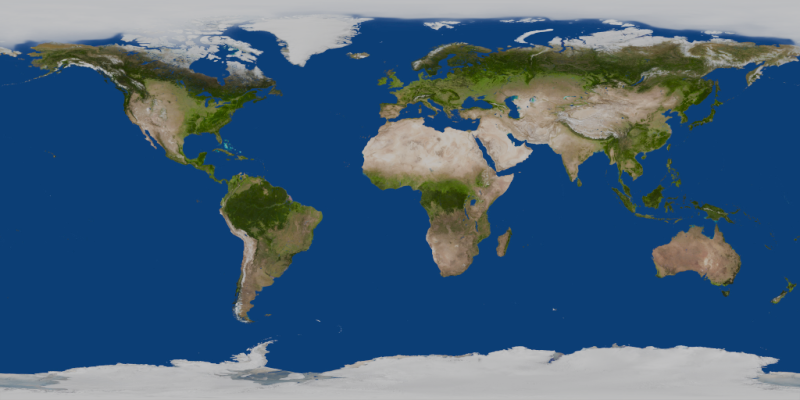
\includegraphics[width=0.6\textwidth]{Imagenes/E4/01_textura_tierra.png}
    \caption{Mapa diurno de la Tierra de Solar System Scope ($2048 \times 1024$, proyección equirrectangular).}
    \label{fig:textura_tierra}
\end{figure}

% ------------------------------------------------------------------------------
\subsection{Actividad 5: Exportación a FBX y carga en OpenGL}

\subsubsection{Exportación}
Las figuras se exportan juntas a \texttt{Blender/escena\_p6.fbx} con \textit{Path Mode} en \textit{Relative}, y las texturas se copian a \texttt{bin/models} junto al FBX, que es donde el cargador las busca. Como \texttt{model.h} ignora la matriz de transformación de cada nodo del FBX (lo comprobamos en la Actividad 2, véase la sección de experimentos), la exportación se hace sobre copias temporales de las mallas con la transformación ya aplicada a los vértices, que se borran al terminar; así el \texttt{.blend} conserva cada objeto con su origen y su posición.

\begin{lstlisting}[language=Python, caption={Exportación con las transformaciones aplicadas a copias temporales (caja\_act2.py).}, label={lst:exportar}]
for ob in originales:
    me = ob.data.copy()
    me.transform(ob.matrix_world)            # posicion final en los vertices
    cp = bpy.data.objects.new(ob.name + "_export", me)
    bpy.context.scene.collection.objects.link(cp)
    copias.append(cp)
...
bpy.ops.export_scene.fbx(filepath=FBX_ESCENA, use_selection=True,
                         path_mode="RELATIVE", object_types={"MESH"})
\end{lstlisting}

\subsubsection{Cambios en el programa}
En \texttt{06\_Texturing.cpp} hicimos cuatro cambios, y uno más en \texttt{model.h}:
\begin{itemize}
    \item El modelo que se carga es \texttt{models/escena\_p6.fbx}, con la rotación de $-90^\circ$ en $X$ que ya traía el código para pasar de $Z$ hacia arriba (Blender) a $Y$ hacia arriba (OpenGL).
    \item El cubo de entorno se dibuja \emph{antes} que el modelo, para que las zonas transparentes de la hoja y de la reja se mezclen con el fondo y no con el color de limpieza.
    \item El \textit{shader} de fragmentos es una copia del original, \texttt{10\_fragment\_alpha.fs}, que además descarta los fragmentos con $\alpha < 0.1$ para que no escriban profundidad (Listado \ref{lst:shader_alpha}). Se dejó como un archivo nuevo para no alterar las demás prácticas, que usan el \textit{shader} original.
    \item La cámara arranca en $(1.5,\ 2.5,\ 14)$ en lugar de $(0,\ 2,\ 10)$, para que al abrir el programa se vean todas las figuras.
    \item En \texttt{model.h} se agregó la bandera \texttt{aiProcess\_GenSmoothNormals} a la lectura del archivo, por la falla que se describe en el experimento de la Actividad 4.
\end{itemize}

\begin{lstlisting}[language=C++, caption={Fragment shader con descarte de fragmentos transparentes (10\_fragment\_alpha.fs).}, label={lst:shader_alpha}]
void main()
{
    vec4 texel = texture(texture_diffuse1, TexCoords);
    if (texel.a < 0.1)
        discard;                    // no escribe color ni profundidad
    vec4 ambientColor = vec4(1.0, 1.0, 1.0, 1.0);
    FragColor = ambientColor * texel;
}
\end{lstlisting}

% ------------------------------------------------------------------------------
\subsection{Actividad 6: Cambio del mapa de entorno}
El manual pide sustituir el fondo por imágenes de Humus \cite{humus}. Al momento de hacer la práctica el sitio \texttt{humus.name} no estaba disponible (el servidor respondía con una página de «sitio no disponible»), así que descargamos el archivo \texttt{Footballfield.zip} desde la copia que guarda el Internet Archive. Escogimos este mapa, una cancha de pasto con cielo nublado, porque combina con las variaciones de la práctica, en particular con el balón y la reja. Sus seis caras miden $2048 \times 2048$ y se distribuyen con licencia CC BY 3.0. La Figura \ref{fig:cruz_football} muestra las seis caras acomodadas en cruz.

\begin{figure}[H]
    \centering
    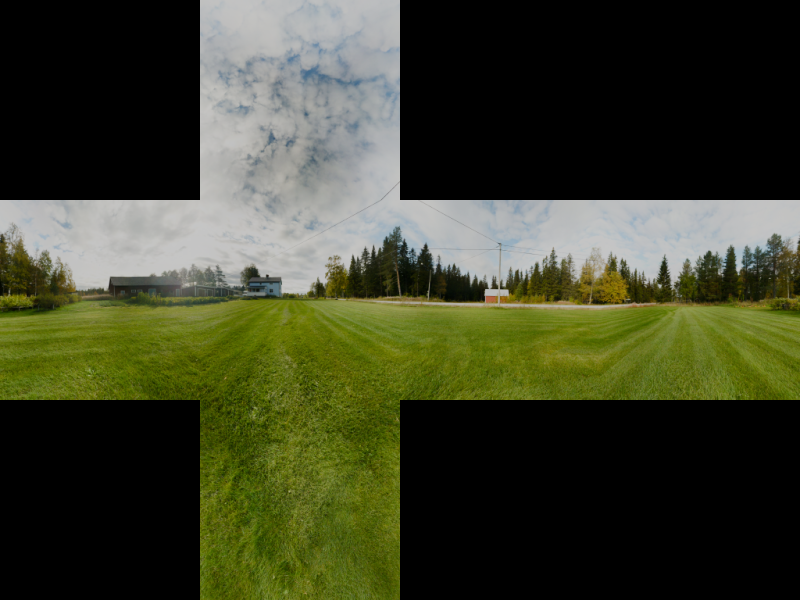
\includegraphics[width=0.6\textwidth]{Imagenes/E6/01_cruz_footballfield.png}
    \caption{Las seis caras del cubemap \textit{Footballfield} de Humus en forma de cruz: \texttt{posy} arriba, \texttt{negy} abajo y, de izquierda a derecha, \texttt{negx}, \texttt{posz}, \texttt{posx} y \texttt{negz}.}
    \label{fig:cruz_football}
\end{figure}

El cubo de entorno del laboratorio (\texttt{mycube.fbx}) tiene seis materiales que buscan sus imágenes con la ruta relativa \texttt{mycube.fbm\textbackslash posx.jpg} y equivalentes. En lugar de sobrescribir esas imágenes, que usan otras prácticas, creamos la carpeta \texttt{bin/models/cubemap\_football} con una copia de \texttt{mycube.fbx} y su propia carpeta \texttt{mycube.fbm} con las seis caras de Humus. Como los dos mapas siguen la misma convención de nombres, cada imagen cae en su cara sin modificar el modelo, y en el código solo cambia la ruta:

\begin{lstlisting}[language=C++, caption={Carga del nuevo mapa de entorno en 06\_Texturing.cpp.}, label={lst:cubemap}]
// Actividad 5.6: cubemap "Footballfield" de Humus (CC BY 3.0)
cubeenv = new Model("models/cubemap_football/mycube.fbx");
\end{lstlisting}

% ------------------------------------------------------------------------------
\subsection{Variaciones: una por cada primitiva}
Además de las actividades del manual, el equipo hizo una variación de cada primitiva, colocadas en una segunda fila detrás de las originales. Todas se generan con el guion \texttt{variaciones.py}.

\subsubsection{Plano: reja de malla ciclónica}
Es un plano de $6 \times 2$ unidades de pie, en $(2, 4.5, 1)$. Su textura RGBA de $1024 \times 1024$ se calcula: el canal alfa vale 1 sobre dos familias de líneas diagonales, $x + y$ y $x - y$ múltiplos de 64 píxeles con un grosor de 3 píxeles, que forman los rombos de la malla; el color es la foto de acero galvanizado \texttt{Metal011}, sombreada con la misma función que el alfa. Un poste vertical al centro y un tubo horizontal arriba, ambos opacos y con sombreado cilíndrico, completan cada tramo. La coordenada $u$ va de 0 a 3 a lo ancho del plano, así que la textura se repite tres veces y la reja tiene tres tramos sin necesidad de una imagen más ancha.

\subsubsection{Cubo: edificio de ladrillo}
Es un cubo escalado a $3 \times 3 \times 6$ unidades con tres pisos de 2 unidades. Su atlas de $2048 \times 2048$ reparte la mitad superior en cuatro fachadas de $512 \times 1024$ (la proporción $1{:}2$ de cada muro) y la mitad inferior en la azotea y la base. Cada fachada combina el ladrillo \texttt{Bricks005} con concreto \texttt{Concrete006} en el zócalo, las losas de cada piso, la cornisa y los marcos de las ventanas, que miden $0.8 \times 1.0$ unidades. Para el vidrio de cada ventana se toma un recorte distinto del cielo del cubemap de Humus, entintado de azul, de modo que las ventanas «reflejan» el mismo cielo del escenario. En la planta baja del frente va una puerta de madera \texttt{Planks012} con su jaladera. La azotea es de concreto con un pretil y un registro.

\subsubsection{Cilindro: tinaco}
Es un cilindro de radio 0.55 y altura 1.1 colocado sobre la azotea del edificio. Su atlas de $1024 \times 1024$ sigue la misma distribución que el del barril: en el costado, el plástico negro \texttt{Plastic006} aclarado para que se noten sus rayones y modulado con $\cos^8$ para formar 7 estrías horizontales, y en la tapa unos anillos concéntricos y la rosca central con 24 crestas.

\subsubsection{Esfera: balón de fútbol}
El patrón de un balón de fútbol es un icosaedro truncado: 12 pentágonos centrados en los vértices de un icosaedro y 20 hexágonos centrados en los vértices del dodecaedro dual. En lugar de dibujarlo a mano, el guion lo calcula para cada píxel de la textura equirrectangular de $2048 \times 1024$: convierte el píxel en la dirección $\mathbf{d}$ con la ecuación de la introducción y busca qué cara toca primero un rayo que sale del centro en esa dirección,
\begin{equation}
    \text{cara}(\mathbf{d}) = \arg\max_i \frac{\mathbf{d} \cdot \mathbf{n}_i}{r_i},
\end{equation}
donde $\mathbf{n}_i$ es el centro unitario de la cara y $r_i$ su distancia al centro del poliedro: $r_p = 2.32744$ para los pentágonos y $r_h = 2.26728$ para los hexágonos, con arista unitaria. Los píxeles en los que las dos mejores caras quedan a menos de 0.0045 se pintan como costura. Los hexágonos llevan el cuero claro \texttt{Leather012} y los pentágonos el mismo cuero oscurecido al 12\,\%. La esfera es de radio 0.6, en $(-5.5, 3, 0.6)$.

\begin{lstlisting}[language=Python, caption={Clasificación de cada píxel del balón en su cara del icosaedro truncado (variaciones.py).}, label={lst:balon}]
normales = np.concatenate([pent / D_PENT, hexa / D_HEX])   # 32 x 3
for f0 in range(0, H, 64):                                  # por bloques de filas
    ...
    d = np.stack([np.cos(lat) * np.cos(lon),
                  np.cos(lat) * np.sin(lon), np.sin(lat)], -1)
    s = d @ normales.T                                      # d . n_i / r_i
    dos = np.partition(s, -2, axis=-1)[..., -2:]
    es_pent[f0:f0 + 64] = s.argmax(-1) < len(pent)
    costura[f0:f0 + 64] = (dos[..., 1] - dos[..., 0]) < 0.0045
\end{lstlisting}
